%!TEX root = ../../super_main.tex
\section{Structural Sensor Data}
\label{sec:structural_sensor_data}

Ideally we want to give the customers the ability to configure their campaigns completely in regards to what and when the outputs from the sensors should be measured. This should be done in such a way that the customers can specify what data is important to them and still avoid draining the resources of the participants devices. For this reason we have designed a way to provide customers with the possibility to configure the temporality of their snapshots. 
\\\\
We go under the assumption that it will be possible to eaves drop in at all times meaning that we can retrieve a measurement from any sensor at all times, however this is not the case but this assumption is enforced as described in \secref{sec:providing_sensor_data}. With the axiom of the sensors we have structured the data from the sensors to be collected as shown in \figref{fig:sample_temporality}. In this figure we see the \emph{measurement} which corresponds to one reading or value of a sensor in a snapshot. Since a single \emph{measurement} from a continuous sensors does not make sense on their own, for instance a single measurement from accelerometer does describe the context in which the participants exist. We introduce a collection of such measurements which we call a \emph{sample}. A \emph{sample} is simply a stream of \emph{measurement}s where the interval or frequency (\emph{measurement frequency}) between them is configurable as seen in \figref{fig:sample_temporality}.

\begin{figure}[!htbp]
    \centering
    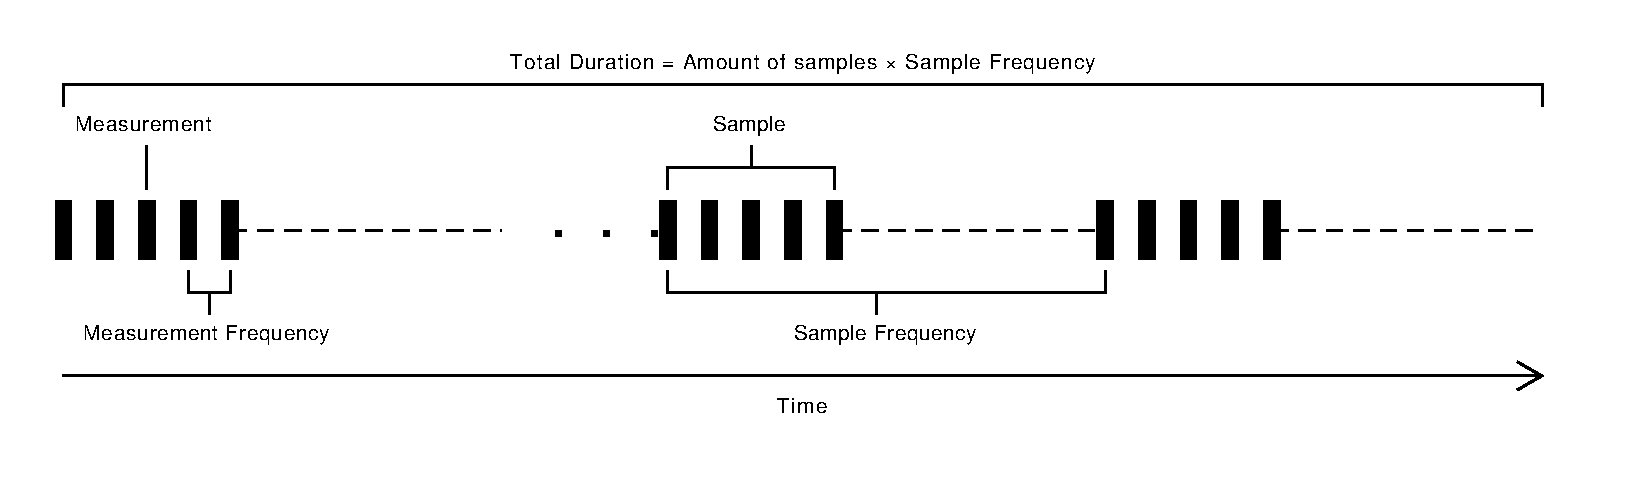
\includegraphics[width=\textwidth]{gathering_sensor_data/sample_temporality.pdf}
    \caption{Temporality of data for a single sensor in a snapshot.}
    \label{fig:sample_temporality}
\end{figure}
\FloatBarrier

Furthermore, we want the customer to configure how often these \emph{sample}s should be gathered, and for that reason we allow them to define a \emph{sample frequency}. And lastly the length of the of the snapshots is configurable by defining a \emph{total duration}, which states for how long the sensor should be measured in total.
\\\\
By this temporal structure of the sensor data we provide a viable way of configuring how the snapshots should be structured in regards to the sensor readings, while maintaining a uniform output format for customers of the system.

\todo[inline]{Vi har reelt 3 forskellige tider: Hvor længe skal et sample vare, hvor ofte skal vi tage et sample, hvor længe skal der gå imellem measurements i et sample? På grund af at sensore i Android giver svar når de har lyst, er det ikke sikkert at der kommer den samme mængde measurements i hver sample. Vi skal overveje om det giver mening, eller om det er vigtigere for kunden at hvert sample med garenti indeholder x measures. Problemet med dette er så at vi ikke kan sætte nogen garenti for hvornår disse measures reelt kommer.}